\chapter{12 апреля. Системы булевых функций}
Операция отрицания $'$ является одной из четырёх булевых функций от одной переменной.

Операция диъюнкции и конъюнкции являются примерами двух из шестнадцати булевых функий от двух переменных, которые перечисляются в следующей таблице:

\begin{adjustbox}{tabular=|c|c|c|c|c|c|c|c|c|c|c|c|c|c|c|c|c|c|,center}
    x & y & $f_1$ & $f_2$ & $f_3$ & $f_4$ & $f_5$ & $f_6$ & $f_7$ & $f_8$ & $f_9$ & $f_{10}$ & $f_{11}$ & $f_{12}$ & $f_{13}$ & $f_{14}$ & $f_{15}$ & $f_{16}$ \\ \hline
    0 & 0 & 0 & 0 & 0 & 0 & 0 & 0 & 0 & 0 & 1 & 1 & 1 & 1 & 1 & 1 & 1 & 1 \\ \hline
    0 & 1 & 0 & 0 & 0 & 0 & 1 & 1 & 1 & 1 & 0 & 0 & 0 & 0 & 1 & 1 & 1 & 1 \\ \hline
    1 & 0 & 0 & 0 & 1 & 1 & 0 & 0 & 1 & 1 & 0 & 0 & 1 & 1 & 0 & 0 & 1 & 1 \\ \hline
    1 & 1 & 0 & 1 & 0 & 1 & 0 & 1 & 0 & 1 & 0 & 1 & 0 & 1 & 0 & 1 & 0 & 1 \\ \hline
    ~ & ~ & 0 & $\cdot$ & $\then'$ & x & $\leftarrow'$ & y & $\oplus$ & + & $\downarrow$ & $\leftrightarrow$ &$y'$ & $\leftarrow$ & $x'$ & $\rightarrow$ & $|$ & $1$
\end{adjustbox}

\begin{itemize}
    \item $x | y$ --- штрих Шеффера
    \item $x \downarrow y$ --- стрелка Пирса
    \item $x \oplus y$ --- функция Жегалкина
    \item $x \leftarrow y$ --- обратная импликация
\end{itemize}

\dftion \textbf{Суперпозицией} булевых функций $g(y_1,~~\dots,~~y_m)$ и $h_1(x_1,~~\dots,~~x_n),$ $\dots,~h_m(x_1, ~~\dots,~~$ $x_n)$ называется булева функция $f(x_1, ~~ \dots,~~$ $x_n)$, значения которой определяются по формуле:
$$f(x_1,\dots,x_n) = g(h_1(x_1,\dots,x_n), \dots, h_m(x_1,\dots,x_n)).$$
Для упрощения записи суперпозиции булевых функций скобки по возможности опускаются с учётом следующего приоритета выполнения булевых операций: $',\cdot$ и затем все остальные операции.

\textbf{Лемма}. Булевы функции от двух переменных взаимосвязаны следующими функциями:
\begin{itemize}
    \item $(x+y)'=x'y'$, $(xy)'=x'+y'$ --- законы де Моргана;
    \item $x+xy=x$, $x(x+y)=x$ --- законы поглощения;
    \item $x+x'=1$, $xx'=0$ --- характеристическое свойство отрицания;
    \item $x+1=1$, $x\cdot 1=x$ --- характеристическое свойство элемента 1;
    \item $x+0=x$, $x\cdot 0 = 0$ --- характеристическое свойство элемента 0;
    \item $x+y=(x'y')', xy=(x'+y')'$ --- взаимосвязь конъюнкции и дизъюнкции;
    \item $x\then y=x'+y$, $x\then y=(xy')'$ --- взаимосвязь импликации с дизъюнкцией, конъюнкцией и отрицанием;
    \item $x \leftrightarrow y = (x \then y)(y \then x)$, $x \leftrightarrow y = (x' + y)(x + y')$
    \item $x | y = (xy)'$, $x'=x|x$, $xy=(x|y)'=(x|y)|(x|y)$, $x+y=x'|y'=(x|x)|(y|y)$ --- взаимосвязь штриха Шеффера с дизъюнкцией, конъюнкцией и отрицанием;
    \item $x\downarrow y = (x+y)', x'=x \downarrow x, x + y = (x \downarrow y)' = (x \downarrow y) \downarrow (x \downarrow y), xy=x'\downarrow y' = (x\downarrow x) \downarrow (y \downarrow y)$ --- взаимосвязь стрелки Пирса с дизъюнкцией, конъюнкцией и отрицанием
\end{itemize}

\dftion \textbf{Суперпозицией} булевых функций $g(y_1,\dots,y_m)$ и $h_1(x_1,\dots,x_n),$ $\dots,h_m(x_1,\dots,x_n)$ называется булева функция $f(x_1, \dots, x_n)$, значения которой определяются по формуле:
$$f(x_1,\dots,x_n) = g(h_1(x_1,\dots,x_n), \dots, h_m(x_1,\dots,x_n)).$$
Для упрощения записи суперпозиции булевых функций скобки по возможности опускаются с учётом следующего приоритета выполнения булевых операций: $',\cdot$ и затем все остальные операции.

\dftion Система булевых функций $F=\{f_1,\dots,f_k\}$ называется \textit{полной}, если любая булева функция может быть представлена в виде суперпозиции функций из этой системы $F$.

\textbf{Теорема Жегалкина}. Любая булева функция $f$ от $n$  переменных представима в виде следующего полинома Жегалкина
$$f(x_1,\dots,x_n) = \underset{(j_1,\dots,j_k)}\oplus x_{i_1}\dots x_{i_k} \oplus c$$
для некоторых хначений $c \in \{0,1\}$ и $1 < i_1 \dots < i_k \leq n$. Причём такое представление булевой функции $f$ единственно с точностью до порядка слагаемых.

\dftion Булева функция $f$ называется \textbf{линейной}, если её представление полиномом Жегалкина не содержит произведения переменных.

Множество всех линейных функций обозначим символом $L$.

\dftion Булева функция $f(x_1,\dots,x_n)$ называется \textit{самодвойственной}, если $f(x_1,\dots,x_n)=(f(x_1',\dots,x_n'))'$.

Множество всех самодвойственных булевых функций обозначим символом $S$.

\dftion Булева функция $f(x_1,\dots,x_n)$ называется монотонной, если $\forall x_1, \dots, x_n, y_1, \dots, y_n \in \{0,1\} \, x_1 \leq y_1, \dots, x_n \leq y_n \then f(x_1,\dots,x_n) \leq f(y_1,\dots,y_n)$

Множество всех монотонных булевых функций обозначим символом $M$.

Пусть $P_0$ --- класс всех булевых функций $f(x_1,\dots,x_n)$, удовлетворяющих условию $f(0,\dots,0)=0$.

Пусть $P_1$ --- класс всех булевых функций $f(x_1,\dots,x_n)$, удовлетворяющих условию $f(1,\dots,1)=1$.

\dftion Классы булевых функций $L, S, M, P_0, P_1$ называются \textit{классами Поста}.

\textbf{Теорема Поста} Система булевых функций в том и только в том случае является полной, если она не содержится ни в одном из классов Поста.

\underline{Алгоритм доказательства полноты системы булевых функций} $F = \{f_1,\dots,f_k\}$:
\begin{enumerate}
    \item Составить таблицу, столбцы которой помечены классами Поста $L, S, M, P_0, P_1$ и строки --- функциями системы $f_1, \dots, f_k$
    \item Для каждой из функций $f_1, \dots, f_k$ проверить принадлежность её к классам Поста и результаты проверки зафиксировать словами <<Да>> <<Нет>> в соответствующей клетке таблицы.
    \item По теореме Поста данная система является полной в том и только в том случае, если в каждом столбце таблицы имеется слово <<Нет>>
\end{enumerate}

\underline{Пример}.

Рассмотрим систему $F\{|\}$, состоящую из одной булевой функции $|$ --- штрих Шеффера. Составляем таблицу, столбцы которой помечены классами Поста $L, S, M, P_0, P_1$ и одна строка --- функцией $|$.

Так как $0|0=1$ и $1|1=0$, функция не принадлежит классам $P_0, P_1$.

В силу свойств $1|0 \neq (0|1)'$, $0|0>1|1$ функция не принадлежит классам $S, M$.

Из равенств $x|y=(xy)'=1\oplus xy$ следует, что функция не принадлежит классу $L$.

Таким образом, по теореме Поста система функций $F=\{|\}$ является полной.

\section{Переключательные схемы}
Рассматриваются электрические ПС, представляющие собой соединённые проводниками переключатели и источники тока.

Условимся обозначать символом 1 протекание тока в проводниках и символом 0 --- отсутствие тока в проводниках.

\begin{figure}[H]
    \centering
    \begin{tikzpicture}[circuit logic IEC,use IEC style logic gates,circuit ee IEC]
        %\tikzset{every node/.style={shape=and gate IEC, logic gate inputs=ini,logic gate input sep=0.5cm}}
        \matrix[column sep=7mm]
        {
                           &                                &                                                                     & \node [logic gate symbol align={bottom, right}, draw] (P2) {$P_2$};  &              & \\
                           &                                & \node [logic gate symbol align={bottom, right}, draw] (P1) {$P_1$}; &                                                                      & \node (c){}; & \\
                           &                                &                                                                     & \node [logic gate symbol align={bottom, right}, draw] (P3) {$P_3$};  &              & \\
            \node (A) {A}; & \node [/tikz/contact] (i) {};  &                                                                     &                                                                      &              & \node [/tikz/contact] (o) {}; & \node (B) {B}; \\
                           &                                & \node [logic gate symbol align={bottom, right}, draw] (P4) {$P_4$}; & \node [logic gate symbol align={bottom, right}, draw] (P5) {$P_5$};  &              & \\
                           &                                &                                                                     &                                                                      &              & \\
        };
        \draw (i.east)  -- ++(right:3mm) |- (P1.west);
        \draw (i.east)  -- ++(right:3mm) |- (P4.west);
        \draw (P1.east) -- ++(right:3mm) |- (P2.west);
        \draw (P1.east) -- ++(right:3mm) |- (P3.west);
        \draw (P2.east) -- ++(right:3mm) |- (c.west);
        \draw (P3.east) -- ++(right:3mm) |- (c.west);
        \draw (c.west)  -- ++(right:3mm) |- (o.west);
        \draw (P4.east) -- ++(right:3mm) |- (P5.west);
        \draw (P5.east) -- ++(right:3mm) |- (o.west);
    \end{tikzpicture}
    \label{fig:ps1}
    \caption{Переключательная схема}
\end{figure}

\dftion \textbf{Переключатель} --- электромагнитное реле с контактами и индукционной катушкой, состояние которой медлируется булевой переменной $x$: $x = 1$ --- в катушке идёт ток, и $x = 0$ --- в катушке тока нет.

Контакты реле --- замыкающие или размыкающие.

Через \textit{замыкающий контакт} реле ток проходит в том и только в том случае, если $x = 1$ --- такой контакт моделируется булевой переменной $x$.

Через \textit{размыкающий контакт} реле ток проходит в том и только в том случае, если $x = 0$ --- такой контакт моделируется отрицанием булевой переменной $x'$.

\underline{Пример}. Пусть в ПС на рис. \ref{fig:ps1} переключатели $P_1, P_5$ имеют общую катушку реле с током $x_1$ и переключатели $P_2, P_4$ имеют общую катущку реле с током $x_2$, причём контакты $P_1, P_2, P_3$ --- замыкающие контакты и контакты $P_3, P_5$ --- размыкающие. Тогда такая ПС с помощью булевых переменных $x_1, x_2, x_3$ изображается следующей диаграммой:

\begin{figure}[H]
    \centering
    \begin{tikzpicture}[circuit logic IEC,use IEC style logic gates,circuit ee IEC]
        %\tikzset{every node/.style={shape=and gate IEC, logic gate inputs=ini,logic gate input sep=0.5cm}}
        \matrix[column sep=7mm]
        {
                                           &                                                               & \node [logic gate symbol align={bottom, right}] (P2) {$x_2$};  &              & \\
                                           & \node [logic gate symbol align={bottom, right}] (P1) {$x_1$}; &                                                                & \node (c){}; & \\
                                           &                                                               & \node [logic gate symbol align={bottom, right}] (P3) {$x_3'$}; &              & \\
            \node [/tikz/contact] (i) {};  &                                                               &                                                                &              & \node [/tikz/contact] (o) {}; \\
                                           & \node [logic gate symbol align={bottom, right}] (P4) {$x_2$}; & \node [logic gate symbol align={bottom, right}] (P5) {$x_1'$}; &              & \\
                                           &                                                               &                                                                &              & \\
        };
        \draw (i.east)  -- ++(right:3mm) |- (P1.west);
        \draw (i.east)  -- ++(right:3mm) |- (P4.west);
        \draw (P1.east) -- ++(right:3mm) |- (P2.west);
        \draw (P1.east) -- ++(right:3mm) |- (P3.west);
        \draw (P2.east) -- ++(right:3mm) |- (c.west);
        \draw (P3.east) -- ++(right:3mm) |- (c.west);
        \draw (c.west)  -- ++(right:3mm) |- (o.west);
        \draw (P4.east) -- ++(right:3mm) |- (P5.west);
        \draw (P5.east) -- ++(right:3mm) |- (o.west);
    \end{tikzpicture}
    \label{fig:ps2}
    \caption{Диаграмма ПС с булевыми переменными}
\end{figure}

Переключатели $p, q$ могут быть соединены последовательно и параллельно.

\begin{figure}[H]
    \centering
    \begin{tikzpicture}[circuit logic IEC,use IEC style logic gates,circuit ee IEC]
        %\tikzset{every node/.style={shape=and gate IEC, logic gate inputs=ini,logic gate input sep=0.5cm}}
        \matrix[column sep=7mm]
        {
             \node [logic gate symbol align={bottom, right}, draw] (p) {$p$}; & \node [logic gate symbol align={bottom, right}, draw] (q) {$q$};  &               \\
        };
        \draw (p.east)  -- ++(right:3mm) |- (q.west);
        \draw (q.east)  -- ++(right:3mm);
        \draw (p.west)  -- ++(left:3mm);
    \end{tikzpicture}
    \begin{tikzpicture}[circuit logic IEC,use IEC style logic gates,circuit ee IEC]
        %\tikzset{every node/.style={shape=and gate IEC, logic gate inputs=ini,logic gate input sep=0.5cm}}
        \matrix[column sep=7mm]
        {
                          & \node [logic gate symbol align={bottom, right}, draw] (P2) {$p$};  &               \\
            \node (P1){}; &                                                                      & \node (c){};  \\
                          & \node [logic gate symbol align={bottom, right}, draw] (P3) {$q$};  &               \\
        };
        \draw (P1.east) -- ++(right:3mm) |- (P2.west);
        \draw (P1.east) -- ++(right:3mm) |- (P3.west);
        \draw (P2.east) -- ++(right:3mm) |- (c.west);
        \draw (P3.east) -- ++(right:3mm) |- (c.west);
        \draw (c.west)  -- ++(right:3mm);
    \end{tikzpicture}
    \label{fig:ps3}
    \caption{Последовательное (слева) и параллельное (справа) соединение}
\end{figure}

Через последовательно соединённые переключатели ток проходит в том и только в том случае, если $p=q=1$ --- такое соединение моделируется булевым многочленом $pq$.

Через параллельно соединённые переключатели $p,q$ ток не проходит в том и только в том случае, если $p=q=0$ --- такое соединение моделируется булевым многочленом $p+q$.

В результате любая электрическая ПС моделируется некоторым булевым многочленом $p$, который принимает значение 1 в том и только в том случае, если в ПС идёт ток.

Соответствующая такому многочлену $p$ булева функция $p$ называется \textit{функцией проводимости} ПС, так как она показывает, при каких значениях булевых переменных (т. е. переключателей данной схемы) в ПС идёт электрический ток.

С другой стороны, каждый раз булев многочлен $p=p(x_1,\dots,x_n)$ моделирует ПС с функцией проводимости $p$: эта схема так конструируется из переключателей $x_1, x_1', \dots, x_n, x_n'$, что в ней при значениях $x_1 = \alpha_1, \dots, x_n = \alpha_n$ проходт ток в том и только в том случае, если $p(\alpha_1, \dots, \alpha_n) = 1$.

\section{Переключательные схемы и логические элементы}
Преключательную схему с функцией проводимости $p=p(x_1,\dots,x_n)$ можно представлять в виде устройства с $n$ входами и одним выходом, которое преобразует входные булевы значения $x_1 = \alpha_1, \dots, x_n = \alpha_n$ в выходное булево значение $\vec p(\alpha_1, \dots, \alpha_n)$.

Графически такое устройство изображается диаграммой в виде прямоугольника с $n$ входами и одним выходом.

\begin{figure}[H]
    \centering
    \begin{tikzpicture}[circuit logic IEC,use IEC style logic gates,circuit ee IEC]
        \matrix[column sep=7mm]
    {
        \node (i0b) {$a_1$}; & \node [/tikz/contact] (i0) {}; &                            & \\
        &                &                            & \\
        \node (i1b) {$a_2$}; & \node [/tikz/contact] (i1) {}; & \node [logic gate symbol align={bottom, right}, draw] (a1) {P};  & \node[/tikz/current direction](o){}; & \node (o2) {$p(\xses[a])$};\\
                        &                            & \\
        \node (i2b) {$a_3$}; & \node [/tikz/contact] (i2) {}; &                            & \\
    };
    \draw (i0.east) -- ++(right:3mm) |- (a1.west);
    \draw (i1.east) -- ++(right:3mm) |- (a1.west);
    \draw (i2.east) -- ++(right:3mm) |- (a1.west);
    \draw (a1.east) -- ++(right:3mm) |- (o.west);
    \end{tikzpicture}
    \label{fig:ps4}
    \caption{}
\end{figure}

Простейшие булевы многочлены моделируют ПС, которые называются \textit{логическими элементами} (или \textit{вентилями}) и обозначаются специальными диаграммами.

\underline{Пример}.

Булев многочлен $p(x)=x'$ моделирует устройство с одним входом и одним выходом и называется NOT-элементом.

\begin{figure}[H]
    \centering
    \begin{tikzpicture}[circuit logic US]
        \matrix[column sep=7mm]
        {
            \node (i1) {$a$}; & \node [/tikz/current direction] (a1) { };  & \node (o) {$a$}; \\
        };
        \draw (i1.east) -- ++(right:3mm) |- (a1.east);
        \draw (a1.west) -- ++(right:3mm) |- (o.west);
    \end{tikzpicture}
\end{figure}


AND-элемент:

\begin{figure}[H]
        \centering
        \begin{tikzpicture}[circuit logic US]
            \matrix[column sep=7mm]
        {
            \node (i0) {$a_1$}; &                            & \\
                            &                            & \\
            \node (i1) {$a_2$}; & \node [and gate,inputs={inini}] (a1) {P};  & \node (o) {$a_1 \cdot a_2 \cdot \dots \cdot a_n$};\\
                            &                            & \\
            \node (i2) {$a_3$}; &                            & \\
        };
        \draw (i0.east) -- ++(right:3mm) |- (a1.input 1);
        \draw (i1.east) -- ++(right:3mm) |- (a1.input 3);
        \draw (i2.east) -- ++(right:3mm) |- (a1.input 5);
        \draw (a1.output) -- ++(right:3mm) |- (o.west);
        \draw (o.east) -- ++(right:3mm);
        \end{tikzpicture}
\end{figure}

OR-элемент:

\begin{figure}[H]
    \centering
    \begin{tikzpicture}[circuit logic US]
        \matrix[column sep=7mm]
    {
        \node (i0) {$a_1$}; &                            & \\
                        &                            & \\
        \node (i1) {$a_2$}; & \node [or gate,inputs={inini}] (a1) {};  & \node (o) {$a_1 + a_2 + \dots + a_n$};\\
                        &                            & \\
        \node (i2) {$a_3$}; &                            & \\
    };
    \draw (i0.east) -- ++(right:3mm) |- (a1.input 1);
    \draw (i1.east) -- ++(right:3mm) |- (a1.input 3);
    \draw (i2.east) -- ++(right:3mm) |- (a1.input 5);
    \draw (a1.output) -- ++(right:3mm) |- (o.west);
    \draw (o.east) -- ++(right:3mm);
    \end{tikzpicture}
\end{figure}

\underline{Пример 1}.
Построим ПС, которая моделирует сложение двух двоичных цифр и называется \textit{полусумматором}. Такая ПС имеет два входа $a_1,a_2$ и два выхода $\vec s(a_1, a_2), \vec c(a_1, a_2)$, которые описывают два разряда суммы $a_1 + a_2$. Таблица этих булевых функций имеет следующий вид:
\begin{figure}[H]
    \centering
    \begin{tabular}{|c|c|c|c|}
        \hline
        $a_1$ & $a_2$ & $\vec s(a_1, a_2)$ & $\vec c(a_1, a_2)$ \\
        \hline
        0     & 0     & 0                  & 0                  \\
        0     & 1     & 1                  & 0                  \\
        1     & 0     & 1                  & 0                  \\
        1     & 1     & 0                  & 1                  \\
        \hline
    \end{tabular}
\end{figure}

Получаем булевы функции:

\begin{itemize}
    \item $c(x_1, x_2) = x_1 \cdot x_2$,
    \item $s(x_1, x_2) = x_1' x_2 + x_2'$,
    \item $s(x_1, x_2) = x_1 \oplus x_2 = (x_1 \leftrightarrow x_2)' = (x_1 \cdot x_2 + x' \cdot x_2') = c' \cdot (x_1 + x_2)$
\end{itemize}

Полусумматор представляется диаграммой:

\begin{figure}[H]
    \centering
    \begin{tikzpicture}[circuit logic US]
    \matrix[column sep=7mm]
    {
        \node (i0) {$a_1$}; &                            & \\
                        & \node [and gate] (a1) {};  & & \node (cdot) {$a_1 \cdot a_2$}; \\
                        &                            & \node [and gate] (o) {}; & \node (oplus) {$a_1 \oplus a_2$}; \\
                        & \node [or gate] (a2) {}; & \\
        \node (i1) {$a_2$}; &                            & \\
    };
    \draw (i0.east) -- ++(right:2mm) |- (a1.input 1);
    \draw (i1.east) -- ++(right:4mm) |- (a1.input 2);
    \draw (i0.east) -- ++(right:2mm) |- (a2.input 1);
    \draw (i1.east) -- ++(right:4mm) |- (a2.input 2);
    \draw (a1.output) -- ++(right:3mm) |- (o.input 1);
    \draw (a2.output) -- ++(right:3mm) |- (o.input 2);
    \draw (a1.output) -- ++(right:3mm) |- (cdot.west);
    \draw (o.output) -- ++(right:3mm);
    \end{tikzpicture}
\end{figure}

Символически полусумматор изображается диаграммой:

\begin{figure}[H]
    \centering
    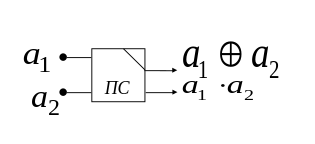
\includegraphics[scale=0.5]{графика/polusum.png}
\end{figure}

\dftion \textit{Сложностью} ПС называется число логических элементов в этой схеме.

Полусумматор реализуется ПС сложности 4.

\textbf{Теорема 1}. Суммирование двух $n$-разрядных двоичных чисел реализуется ПС сложности $9n-5$, которая обозначается $S_n$ и называется \textit{сумматором} порядка $n$.

\textbf{Теорема 2}. Умножение двух $n$-разрядных двоичных чисел реализуется ПС сложности $O(n^{log_2 3})$, которая обозначается $M_n$ и называется \textit{умножителем} порядка $n$.